\documentclass{beamer}
\usetheme{EastLansing}\usecolortheme{crane}
\usefonttheme{professionalfonts}\useinnertheme{rectangles}
%-----------------------------------------------------------------------------%
\usepackage{settings}
%-----------------------------------------------------------------------------%
%%% Title %%%
\title{Chapter 5: Growing Random Networks}
\subtitle{Social and Economic Networks, Matthew O.\ Jackson}
\author{陳\ 捷}
\date{\texttt{2023-02-11}}
%-----------------------------------------------------------------------------%

\begin{document}

\begin{frame}{}
	\maketitle
\end{frame}

\begin{frame}{Roadmap}
	\tableofcontents
\end{frame}

\begin{frame}{Recap and Introduction}
	We considered ``random graph-based models'' last week,
	so why consider ``growing networks''?
	\begin{enumerate}
		\item
			In many applications, it is more natural to consider \emph{growing} networks.
			\begin{itemize}
				\item web pages, scientific journals (citations)
				\item people entering new environments (e.g., schools, workplaces, neighbourhoods, cities)
			\end{itemize}
		\item
			Growing models provide extra richness to the model that is not present in Poisson random networks. \\
			That is, with the \textbf{time dimension} now in consideration,
			we can model features such as \emph{fat-tailedness} and \emph{clustering} naturally.
	\end{enumerate}
\end{frame}

\section{Uniform Randomness}

\begin{frame}{Notation}
	\begin{itemize}
		\item
			Discrete time: $t\in\{0,1,2,...\}$.
		\item
			One node is born at each time, and the node is named after its birth date.
		\item
			Let $\yellow{d}_{\red{i}}(\blue{t})$ denote the \yellow{degree} (undirected unless specified) of \red{node $i$} at \blue{time $t$}.
	\end{itemize}
\end{frame}

\begin{frame}{Exponential Model (Uniform Randomness)}
	\begin{itemize}
		\item
			At the birth of each node,
			it connects to $m$ other nodes randomly (uniformly).
		\item
			We want to derive the (asymptotic) \emph{degree distribution} of this model setting.
	\end{itemize}
\end{frame}

\begin{frame}{Degree Distribution of Exponential Model}
	\begin{itemize}
		\item
			For the model to be well-defined,
			we assume that we are starting with a $m$-node clique.
			This assumption will not affect the degree distribution in the limit.
		\item
			Thus, the first new born node is $m+1$.
		% \item
		% 	At time $m+2$,
		% 	each preexisting node expects to gain $m/(m+1)$ links.
		\item
			At time $t$,
			each node $i\in\{m+1,...,t\}$ has \textbf{expected} links
			\begin{align*}
				m+\frac{m}{i+1}+\cdots+\frac{m}{t}
				\approx
				m\left(1+\ln(t)-\ln(i)\right)
			\end{align*}
		\item
			Given a degree $d$ at time $t$,
			nodes that have expected degree less than $d$ are those such that
			\begin{align*}
				m\left(1+\ln(t)-\ln(i)\right) < d
				\implies i > t\exp\left(1-\frac{d}{m}\right),
			\end{align*}
			i.e., nodes that are born after $t\exp(1-d/m)$.
	\end{itemize}
\end{frame}

\begin{frame}{Degree Distribution of Exponential Model (cont'd)}
	\begin{itemize}
		\item
			Hence, the fraction of nodes that have expected degree less than $d$ is
			\begin{align*}
				\frac{t\exp\left(1-\frac{d}{m}\right)}{t}
				= \exp\left(1-\frac{d}{m}\right)
			\end{align*}
		\item
			Therefore, the expected degree distribution is
			\begin{align}\label{eq:degree_distribution_direct}
				F_t(d)
				= 1 - \exp\left(1-\frac{d}{m}\right)
			\end{align}
			This is a variation of an exponential distribution.
			% TODO: mean of 2m
	\end{itemize}
	\begin{block}{Note}
		\begin{itemize}
			\item The distribution is time-independent. This is not true in general.
			\item We are using \textbf{expected} degree to obtain the distribution.
		\end{itemize}
	\end{block}
\end{frame}

\subsection{Mean-Field Approximation} % TODO

\begin{frame}{Mean-Field Approximations}
	The technique we used (using expected degree) is called \textbf{mean-field approximation}.
	\begin{itemize}
		\item
			The burning question is: \textbf{Is this approximation good for ``actual'' degrees?}
		\item
			For simple models, such as the exponential model and the preferential attachment model, we know this approximation is correct.
		\item
			However, the answer is \shruggie\ most of the time.
		\item
			The next-best thing to do is use simulation to check whether the approximation is good.
	\end{itemize}
\end{frame}

% TODO: difference with Poisson networks

\subsection{Continuous Time Approximation of Degree Distribution}

\begin{frame}{Degree Distribution of Exponential Model (Conti.\ time)}
	\begin{itemize}
		\item
			Now we consider a \emph{continuous time view} to approximating the degree distribution.
		\item
			A node starts with $d_{i}(t=i)=m$;
			then, the node gains $m/t$ links in expectation at any time $t$ after $i$.
		\item
			This description yields an differential equation
			\begin{align*}
				\D{t}{d_{i}(t)} = \frac{m}{t}.
			\end{align*}
		\item
			This differential equation has a solution
			\begin{align*}
				d_{\red{i}}(\blue{t}) = m+m\ln\left(\frac{\blue{t}}{\red{i}}\right)
			\end{align*}
		\item
			Note that $d_{i}(t)$ is decreasing in $\red{i}$ and increasing in $\blue{t}$.
			This fits the intuition that older nodes have higher degrees.
	\end{itemize}
\end{frame}

\begin{frame}{Degree Distribution of Exponential Model (Continued)}
	\begin{itemize}
		\item
			Let $i_{t}(d)$ denote a node such that \red{node $i_{t}(d)$} has \yellow{degree $d$} at \blue{time $t$},
			i.e., $d_{\red{i_{t}(d)}}(\blue{t})=\yellow{d}$.
		\item
			Since $d_{i}(t)$ is decreasing in $i$, ...
			\begin{enumerate}
				\item $i_{t}(d)$ is well-defined,
				\item only the nodes born after $i_t(d)$ have degrees less than $d$.
			\end{enumerate}
		\item
			In our case, $i_{t}(d)$ assumes the form
			\begin{align*}
				i_{t}(d) = t\exp\left(1-\frac{d}{m}\right)
			\end{align*}
		\item
			Hence, the resulting degree distribution is
			\begin{align*}
				F_{t}(d)
				= 1 - \frac{i_{t}(d)}{t}
				= 1 - \exp\left(1-\frac{d}{m}\right),
			\end{align*}
			which is identical to what we have obtained \hyperlink{eq:degree_distribution_direct}{earlier}.
	\end{itemize}
\end{frame}

\begin{frame}{Degree Distribution of Exponential Model (Continued)}
	\begin{block}{Remarks}
		Solving first order ODE's has several advantages:
		\begin{enumerate}
			\item
				It is often simpler than the direct method.
			\item
				It can make model specification simpler,
				as we only have to specify (1) the initial condition of $d_{i}(t)$ at $t=i$ and
				(2) how $d_{i}(t)$ evolves through time.
		\end{enumerate}
	\end{block}
	\begin{itemize}
		\item
			Continuous time approximation is not a big problem.
			It is relatively minor and it smooths things out.
		\item
			The main problem of approximating the degree distribution is still
			the discrepancy between ``expected degrees'' and ``actual degrees''.
	\end{itemize}
\end{frame}

\section{Preferential Attachment}

\begin{frame}{Preferential Attachment} % TODO: intro to Preferential Attachment
	\begin{itemize}
		% \item
		% 	With the techniques of approximating the degree distribution,
		% 	we now turn to another network formation process: \textbf{preferential attachment}.
		\item
			\textbf{Motivation}:
			New comers do not form links with existing members \emph{at random}.
			More likely, they form links with existing members that has a lot of connections already.
		\item
			The two main ingredients of this process is
			\begin{enumerate}
				\item The system grows over time.
				\item The existing objects grow at rates proportional to their size.
			\end{enumerate}
			These two properties leads to \textbf{scale-free distributions}.
		\item
			Many big names studied this phenomenon:
			\begin{itemize}
				\item Pareto (1896): wealth distribution (Pareto distribution)
				\item Yule (1925): explain the distribution of city sizes
				\item Zipf (1949): word frequency (Zipf's law)
				\item Simon (1995): formalize processes that generates scale-free distributions
				\item Price (1965): citation network
			\end{itemize}
	\end{itemize}
\end{frame}

\begin{frame}{Degree Distribution of Preferential Attachment}
	\begin{itemize}
		\item
			Each newborn node still forms $m$ links,
			but not uniformly across existing nodes.
		\item
			Each new node links to a preexisting node with probabilities proportional to their degrees,
			i.e., an existing node $i$ is expected to get
			\begin{align*}
				m \frac{d_{i}(t)}{\yellow{\sum_{j=1}^{t}d_{j}(t)}}
				= m \frac{d_{i}(t)}{\yellow{2tm}}
				= \frac{d_{i}(t)}{2t}
			\end{align*}
			links from the newborn node at time $t$.
		\item
			Thus, the mean-field, continuous-time approximation of this process is
			\begin{align*}
				\D{t}{d_{i}(t)} = \frac{d_{i}(t)}{2t}
			\end{align*}
			with initial condition $d_{i}(t=i)=m$.
	\end{itemize}
\end{frame}

\begin{frame}{Degree Distribution of Preferential Attachment (Cont'd)}
	\begin{itemize}
		\item
			A solution to the ODE is
			\begin{align*}
				\yellow{d}_{\red{i}}(\blue{t}) = m\left(\frac{\blue{t}}{\red{i}}\right)^{1/2}
				\quad\leadsto\quad
				\red{i}_{\blue{t}}(\yellow{d}) = \blue{t}\left(\frac{m}{\yellow{d}}\right)^{2}.
			\end{align*}
		\item
			Hence, the degree distribution is
			\begin{align*}
				F_{t}(d)
				= 1 - \frac{i_{t}(d)}{t}
				= 1 - \left(\frac{m}{d}\right)^{2}
			\end{align*}
			The corresponding density function is
			\begin{align*}
				f_{t}(d) = 2m^{2} d^{-3}.
			\end{align*}
	\end{itemize}
	\begin{block}{}
		Thus, the preferential attachment process naturally motivates a \textbf{scale-free distribution}
		with exponent $3$. (scale-free distribution: $p(d) = cd^{-3}$)
	\end{block}
\end{frame}

\begin{frame}{Comparison of Preferential Attachment and Exponential Model}
	\begin{center}
		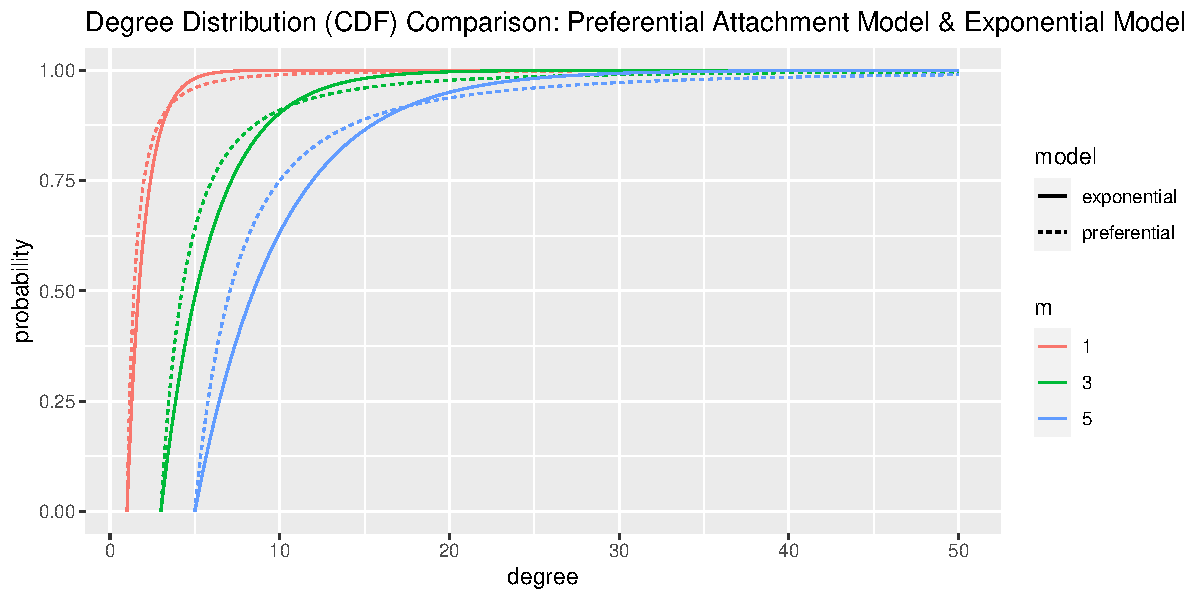
\includegraphics[width=\textwidth]{figures-R/comparison-cdf.pdf}
	\end{center}
\end{frame}

\subsection*{Motivating a Different Exponent}

\begin{frame}{Motivating a Different Exponent}
	\begin{itemize}
		\item
			The exponent $3$ comes from the fact that $\sum_{j=0}^{t}d_{j}(t)=2tm$.
			% TODO: more explanation.
		\item
			Thus, if we specify the differential equation more generally thus
			\begin{align*}
				\D{t}{d_{i}(t)} = \frac{d_{i}(t)}{\gamma t},
			\end{align*}
			the corresponding degree distribution would be
			\begin{align*}
				f_{t}(d) = \gamma m^{\gamma} d^{-\gamma-1}.
			\end{align*}
		\item
			Intuitively,
			the growth of $d_{i}(t)$ is proportional to itself (the main feature of preferential attachment)
			and is scaled by a factor of $\gamma^{-1}$.
			The smaller $\gamma$ is, the faster $d_{i}(t)$ grows over time,
			which leads to a fatter tail.
	\end{itemize}
\end{frame}

\begin{frame}{Motivating a Different Exponent (Cont'd)}
	\begin{center}
		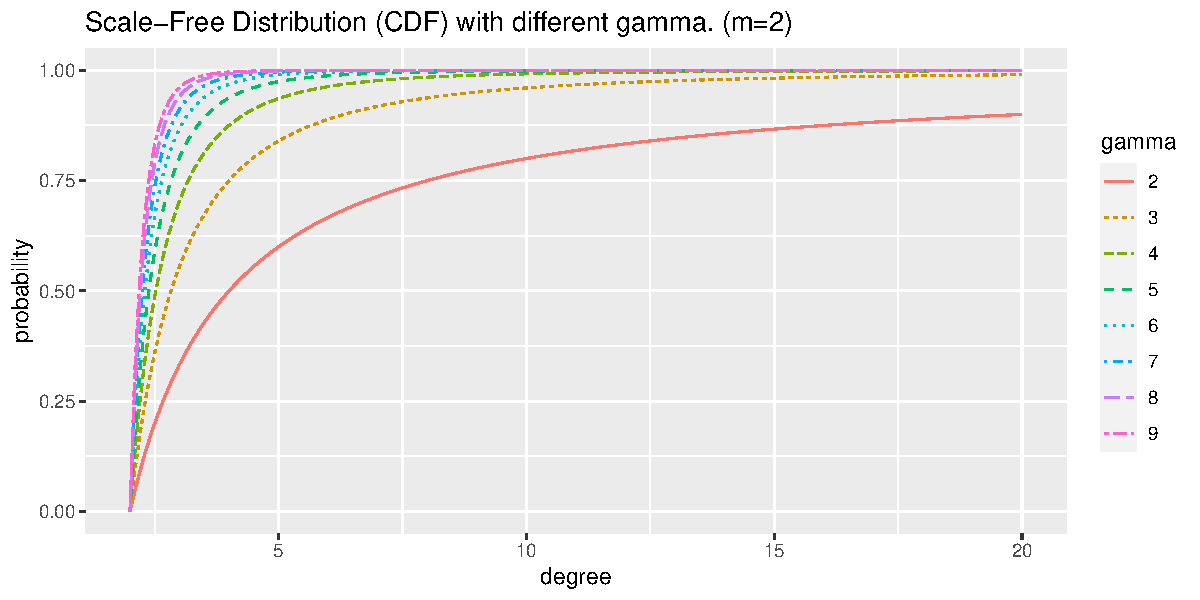
\includegraphics[width=\textwidth]{figures-R/scalefree_distribution-cdf.pdf}
	\end{center}
\end{frame}

\begin{frame}{Motivating a Different Exponent (Cont'd)}
	\begin{itemize}
		\item
			It is not very straight forward to justify/motivate a $\gamma$ that is not $2$.
		\item
			A possible motivation is thus:
			\begin{itemize}
				\item
					At each time period, a group of nodes are born.
				\item
					In the same period, $m$ new connects are created.
				\item
					Of the $m$ connects,
					$\alpha m$ are made to existing nodes, and
					$(1-\alpha) m$ are made within the new nodes.
			\end{itemize}
		\item
			In this setting,
			an existing node $i$ is expected to get
			\begin{align*}
				\alpha m \frac{d_{i}(t)}{2mt}
				= \alpha \frac{d_{i}(t)}{2t}
				= \frac{d_{i}(t)}{(2/\alpha)t}
			\end{align*}
			new links.
			Here, $\gamma=2/\alpha$.
	\end{itemize}
\end{frame}

\section{Hybrid Models}

\begin{frame}{Real Data}
	\begin{itemize}
		\item
			Co-authorship data fits between a uniformly random network and a preferential attachment network.
			That is, the data has a fat tail, but less fat than preferential attachment network.
	\end{itemize}
	\begin{center}
		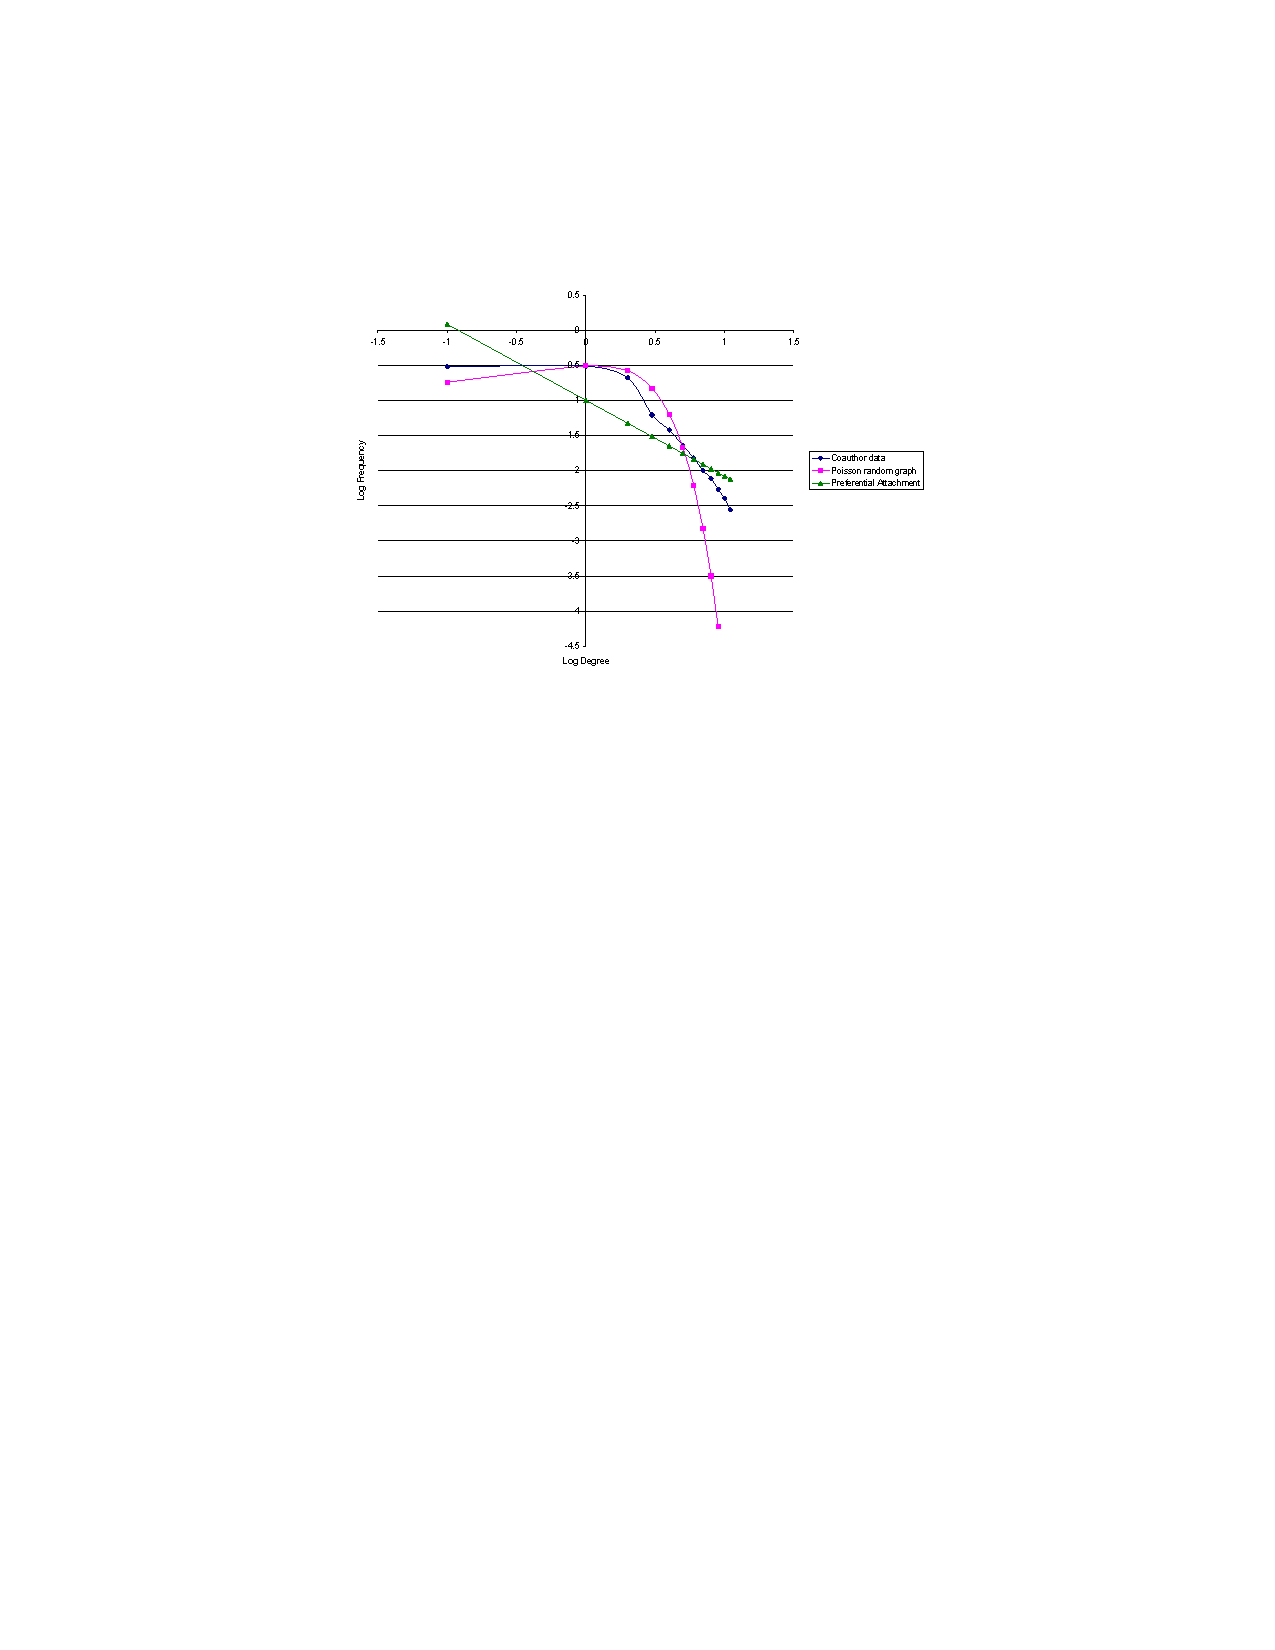
\includegraphics[width=0.6\textwidth]{figures/coauthor_data.pdf}
	\end{center}
	\begin{itemize}
		\item
			Thus, we are motivated to build a hybrid model.
	\end{itemize}
\end{frame}

\subsection*{Mixing Random and Preferential Attachment}

\begin{frame}{Hybrid Model}
	\begin{itemize}
		\item
			We can intuitively build a hybrid model:
		\item
			Each new node form $m$ connections,
			of which $m\alpha$ links randomly to existing nodes and
			of the rest $m(1-\alpha)$ links to existing node via preferential attachment:
			\begin{align*}
				\D{t}{d_{i}(t)} = \alpha\frac{m}{t} + (1-\alpha)\frac{d_{i}(t)}{2t}
			\end{align*}
		\item
			The ODE has solution
			\begin{align*}
				d_{\red{i}}(\blue{t})
				= \left(m+\frac{2\alpha m}{1-\alpha}\right)\left(\frac{\blue{t}}{\red{i}}\right)^{(1-\alpha)/2}
				- \frac{2\alpha m}{1-\alpha}
			\end{align*}
		\item
			The degree distribution is
			\begin{align}\label{eq:hybrid_cdf}
				F_{t}(d)
				= 1 - \frac{i_{t}(d)}{t}
				= 1 - \left(\frac{m+\frac{2\alpha m}{1-\alpha}}{d+\frac{2\alpha m}{1-\alpha}}\right)^{\frac{2}{1-\alpha}}
			\end{align}
	\end{itemize}
\end{frame}

\subsection*{Simulation as a Check on the Degree Distribution}

\begin{frame}{Hybrid Model (Simulation)}
	\begin{center}
		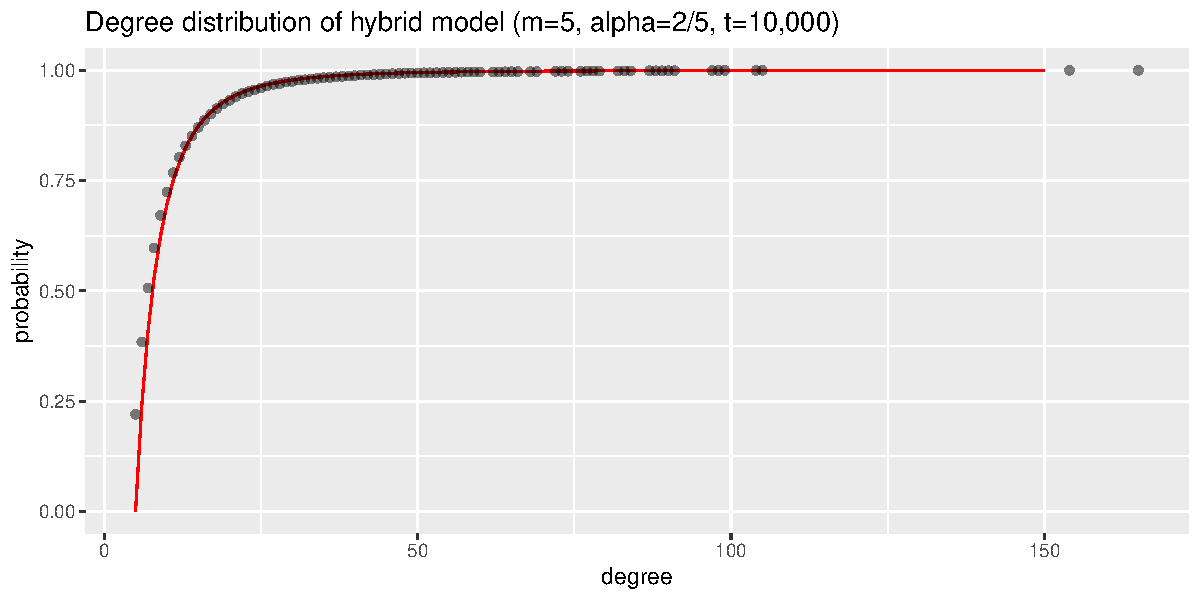
\includegraphics[width=\textwidth]{figures-R/hybrid-cdf.pdf}
	\end{center}
\end{frame}

\begin{frame}{Hybrid Model (Simulation, Cont'd)}
	\begin{center}
		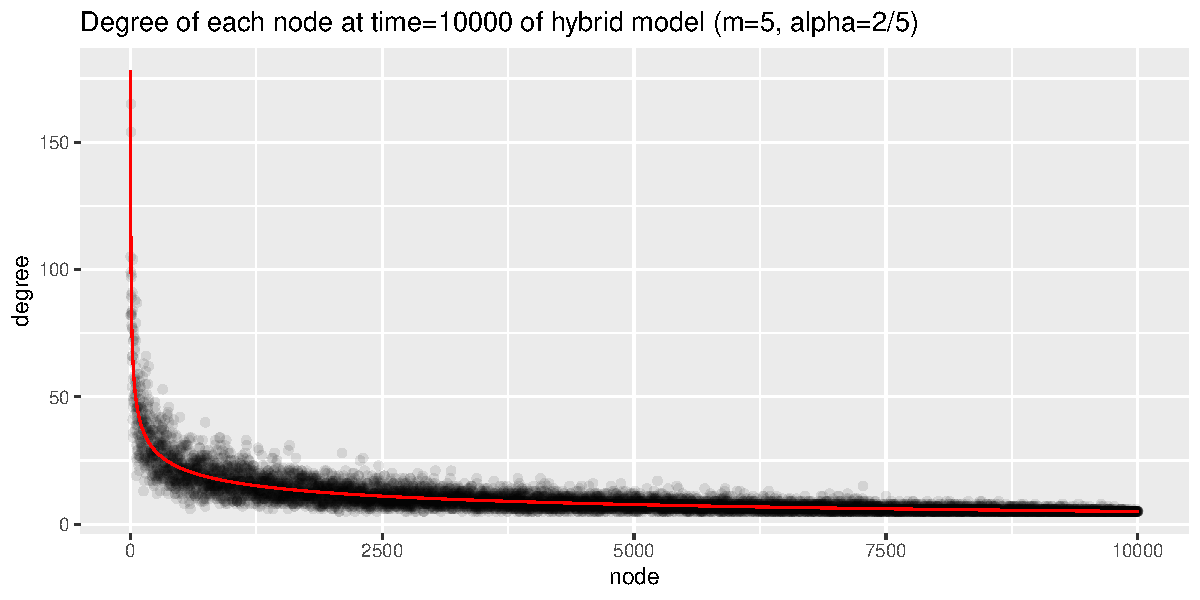
\includegraphics[width=\textwidth]{figures-R/hybrid-degree.pdf}
	\end{center}
\end{frame}

\subsection*{Fitting Hybrid Degree Distribution to Data}

\begin{frame}{Fitting the Hybrid Model}
	\begin{itemize}
		\item
			The parameter $\alpha$ is interesting,
			since it can be interpreted as the proportion that the network formation process is through uniform randomness/preferential attachment.
		\item
			Parameter $m$ can be observed directly by dividing the total degree by $2t$.
			Many methods can be used to estimate the CDF:
			\begin{align*}
				\ln(1-F(\yellow{d}))
				= \frac{2}{1-\grey{\alpha}}\ln\left(m+\frac{2\grey{\alpha} m}{1-\grey{\alpha}}\right)
				- \frac{2}{1-\grey{\alpha}}\ln\left(\yellow{d}+\frac{2\grey{\alpha} m}{1-\grey{\alpha}}\right)
			\end{align*}
		\item
			Fitting this model to co-authorship data listed on \href{https://www.aeaweb.org/econlit/}{EconLit} during 1990's yields an estimation of $\hat\alpha=0.56$.
			(Goyal, van der Liej, Moraga-Gonzalez, 2006)
	\end{itemize}
\end{frame}

\section{Other Aspects of a Growing Network}

\begin{frame}{}
	Now we take a look at other aspects of a network.
	\begin{itemize}
		\item \hyperlink{sec:diameter}{Diameter}
		\item \hyperlink{sec:assortativity}{Positive Assortativity}
		\item \hyperlink{sec:clustering}{Clustering}
	\end{itemize}
\end{frame}

\subsection{Diameter}\label{sec:diameter}

\begin{frame}{Diameter}
	\begin{itemize}
		\item
			In general, the diameter (or average path length) of a network is very difficult to calculate beyond Poisson random graph.
		\item
			Intuitively, a model with preferential attachment should have lower diameter (compared to a Poisson graph),
			since there high degree nodes serves as hubs.
	\end{itemize}
	\begin{block}{Theorem (Bollob\'{a}s \& Riordan, 2004)}
		Consider a preferential attachment model where each newborn node forms $m\geq 2$ links.
		As $t$ increases,
		the resulting graph will consist of a single component with diameter proportional to $\frac{\log{t}}{\log\log{t}}$ almost surely.
	\end{block}
	\begin{itemize}
		\item
			The diameter of a Poisson network is proportional to $\log{t}$ if the average degree is fixed.
	\end{itemize}
\end{frame}

\subsection{Positive Assortativity and Degree Correlation}\label{sec:assortativity}

\begin{frame}{Positive Assortativity and Degree Correlation}
	\begin{block}{Assortativity}
		a preference for a network's nodes to attach to others that are \emph{(dis)similar} in some way.
		(選擇性、選型性、同配性)
	\end{block}
	\begin{itemize}
		\item
			Many networks exhibits positive assortativity,
			a feature absent in Poisson graphs.
	\end{itemize}
	\begin{block}{Theorem (Jackson \& Rogers, 2007b)}
		Consider a hybrid model.
		Under mean-field estimation,
		the \blue{estimated distribution of $i$'s neighbors' degree} strictly \hyperlink{app:FSD}{first-order stochastically dominates}
		that of $j$'s at each $t>j$ for all $j>i$.
		In particular, $\blue{F^{t}_{i}(d)}<F^{t}_{j}(t)$ for all $d<d_{i}(t)$.
	\end{block}
	\begin{itemize}
		\item
			This means, an older node has friends that have more connections.
	\end{itemize}
\end{frame}

\subsection{Clustering in Growing Random Networks}\label{sec:clustering}

\begin{frame}{Clustering}
	\begin{itemize}
		\item
			Clustering is another idea that is observed in reality but not captured by Poisson graphs.
		\item
			Even in a exponential graph or hybrid models,
			clustering is not captured.
			That is, clustering converges to $0$ as $t\to\infty$.
		\item
			Intuitively, the probability of forming clusters is too low in exponential graphs.
			The probability of two new links creasting a cluster is
			\begin{align*}
				\frac{tm\ \text{(all existing links)}}{{t\choose2}\ \text{(all pairs of nodes)}}
				= \frac{2m}{t-1}
				\to 0
				\quad\text{as}\quad
				t\to\infty.
			\end{align*}
		\item
			\textbf{Idea}: For a model to capture ``clustering'',
			the network formation process has to depend on ``the existing graph structure''
			rather than only on the degree.
	\end{itemize}
\end{frame}

\begin{frame}{A Meeting-Based Network Formation Model}
	\begin{center}
		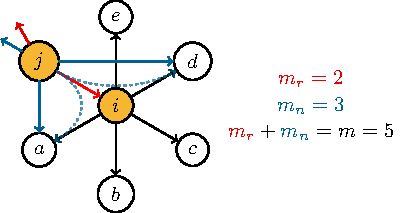
\includegraphics[scale=1]{figures-tikz/meeting_basted_network.pdf}
	\end{center}
	\begin{itemize}
		\item
			A new node ($j$) is born.
			Let $m=\red{m_{r}}+\blue{m_{n}}$.
		\item\textbf{Step 1}:
			Pick $\red{m_{r}}$ nodes randomly to link to.
			($j$ picks $i$ in this step)
		\item\textbf{Step 2}:
			Randomly choose $\blue{m_{n}}$ of the \emph{out-links} of the $\red{m_{r}}$ nodes and link to the corresponding nodes,
			i.e., linking to ``friends of friends.''
			($j$ picks $2$ of out-links of $i$ and links to corresponding node $a$ and node $d$)
	\end{itemize}
\end{frame}

\begin{frame}{}
	\begin{itemize}
		\item
			Thus, we have the following ODE characterizing the change in in-degree:
			\begin{align*}
				\D{t}{d_{i}^{\text{in}}(t)}
				= \underbrace{\red{\frac{m_{r}}{t}}}_{\text{\textbf{Step 1}}}
				+ \underbrace{\blue{\frac{m_{r}d_{i}^{\text{in}}(t)}{t} \frac{m_{n}}{m_{r}m}}}_{\text{\textbf{Step 2}}}
				&= \frac{m_{r}}{t}
				+ \frac{m_{n}d_{i}^{\text{in}}(t)}{mt} \\
				&= \underbrace{\frac{m_{r}}{m}}_{\alpha} \frac{m}{t}
				+ \underbrace{\frac{m_{n}}{m}}_{1-\alpha} \frac{d_{i}^{\text{in}}(t)}{t}
			\end{align*}
			with initial condition $d_{i}^{\text{in}}(i)=0$.
			% Note that $d_{i}^{\text{out}}(t)=m$ $\forall t$.
		\item
			The resulting in-degree distribution is
			\begin{align*}
				% F(d^{\text{in}}) = 1 - (rm)^{1+r} (d^{\text{in}}+rm)^{-(1+r)}
				F(d^{\text{in}}) = 1 - \left(\frac{rm}{d^{\text{in}}+rm}\right)^{1+r}
			\end{align*}
			where $r=m_r/m_{n}$. \hyperlink{eq:hybrid_cdf}{\beamerreturnbutton{compare}}
	\end{itemize}
\end{frame}

\begin{frame}{Discussion of Meeting-Based Network}
	\begin{enumerate}
		\item
			The reason we consider a directed network here is for the tractability of \textbf{Step 2}.
			\begin{itemize}
				\item
					In our case, $d_{t}^{\text{out}}(t)=m$ $\forall t$ makes the calculation easy.
				\item
					In an undirected network,
					it is hard to count the total degree of the $\red{m_{r}}$ chosen nodes.
			\end{itemize}
		\item
			A directed network with constant out-degree might be a good model for webpages or scientific articles,
			but not for human interactions.
		% \item
		% 	Also, in an undirected network,
		% 	it is possible that the node found in \textbf{Step 2} is already chosen in \textbf{Step 1}.
	\end{enumerate}
\end{frame}

\begin{frame}{Clustering}
	\begin{center}
		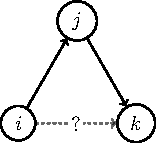
\includegraphics[scale=1]{figures-tikz/transitive.pdf}
	\end{center}
	\begin{itemize}
		\item
			Now we consider the property of interest: \emph{clustering}.
		\item
			Recall that \textbf{transitive triple clustering measure} is
			\begin{align*}
				\clustertt(g) = \frac{\sum_{i;j\neq i;k\neq j}g_{ij}g_{jk}g_{ik}}{\sum_{i;j\neq i;k\neq j}g_{ij}g_{jk}}
			\end{align*}
		\item
			Clearly,
			this model is designed in a way such that transitive triples are common.
			But how common exactly?
	\end{itemize}
\end{frame}

\begin{frame}{}
	\begin{center}
		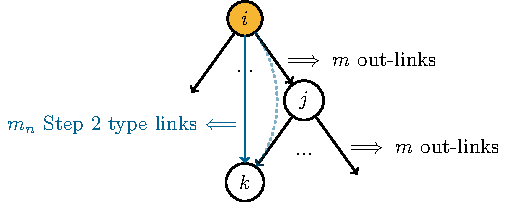
\includegraphics[scale=1]{figures-tikz/clustering.pdf}
	\end{center}
	\begin{itemize}
		\item
			The denominator of $\clustertt(g)$ is $tm^2$.
		\item
			The nominator of $\clustertt(g)$ is ``at least'' $tm_{n}$.
		\item
			Thus, the lower-bound of $\clustertt(g)$ is
			\begin{align*}
				\frac{tm_{n}}{tm^{2}}
				= \frac{m_{n}}{m^{2}}
				= \frac{1}{(1+r)m}
			\end{align*}
			where $r=m_{r}/m_{n}$.
		\item
			This lower-bound turn out to be the correct $\clustertt$ when $r\geq1$.
	\end{itemize}
\end{frame}

\begin{frame}{}
	\begin{itemize}
		\item
			In order to simplify the calculation,
			consider a special process:
			\begin{itemize}
				\item
					when $r\geq1$,
					then at most one link is formed in each node found in \textbf{Step 1}.
				\item
					when $r<1$,
					then exactly $m_{n}/m_{r}$ are formed in each node found in \textbf{Step 1}.
			\end{itemize}
		\item
			The parameter $r<1$ means that more than half of the friends made by a new node are ``friends of friends''.
			This means any link created in \textbf{Step 2} is very likely to generate more than one transitive triple.
	\end{itemize}
	\begin{block}{Proposition (Jackson \& Rogers, 2007b)}
		Under a mean-field approximation specified above,
		the fraction of transitive triples, $\clustertt$, tends to
		\begin{align*}
			\begin{cases}
				\frac1{(1+r)m} & \text{ if } r\geq 1, \\
				\frac{r(m-1)}{m(m-1)(1+r)r - m(1-r)} & \text{ if } r < 1.
			\end{cases}
		\end{align*}
	\end{block}
\end{frame}

\begin{frame}{}\label{fig:clustering-estimation}
	\begin{center}
		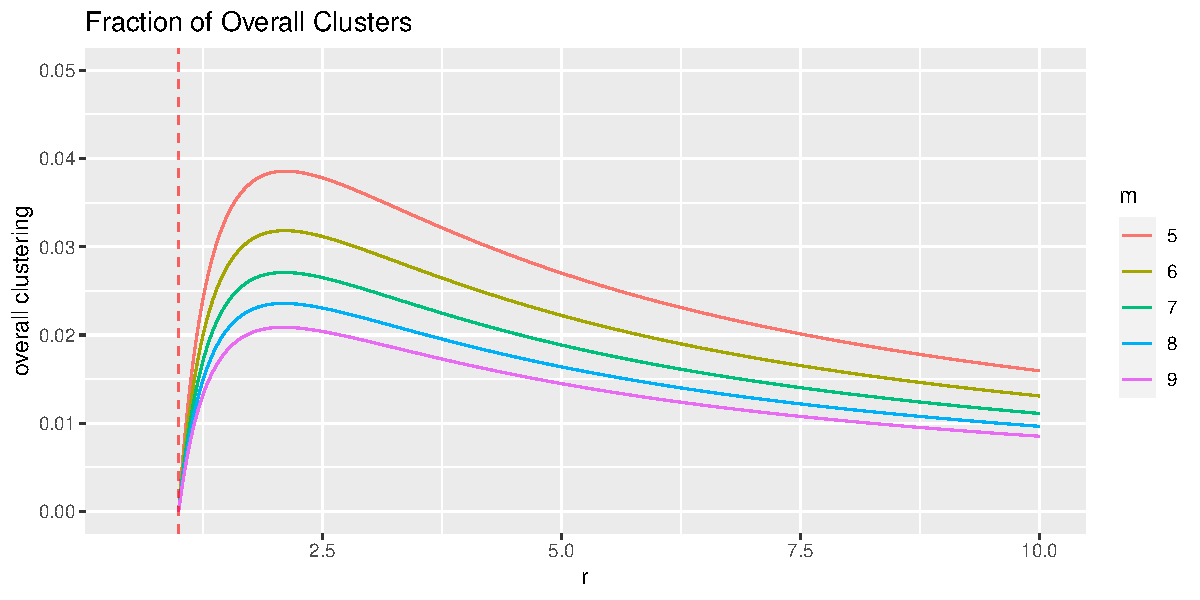
\includegraphics[width=\textwidth]{figures-R/clustering-estimation.pdf}
	\end{center}
	\begin{itemize}
		\item
			There is actually a kink at $r=1$.
	\end{itemize}
\end{frame}

\begin{frame}{Example: Case $r<1$}
	\begin{center}
		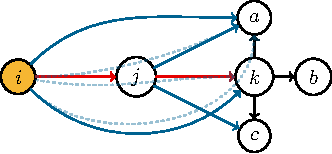
\includegraphics[scale=1]{figures-tikz/r_leq_1.pdf}
	\end{center}
	\begin{itemize}
		\item
			Consider the case where $\red{m_{r}=1}$ and $\blue{m_{n}=2}$.
		\item
			Previously, node $j$ connects to $k$ in \textbf{Step 1}
			and connects to $a$ and $c$ in \textbf{Step 2}.
		\item
			Now, a new node $i$ connects to $j$ in \textbf{Step 1},
			then it connects to $a$ and $k$ in \textbf{Step 2}.
		\item
			In this case, $3$ transitive triples are generated instead of $2$.
			\begin{itemize}
				\item $i\to j\to a$ $\implies$ $i\to a$.
				\item $i\to j\to k$ $\implies$ $i\to k$.
				\item $i\to k\to a$ $\implies$ $i\to a$. (This triple we did not expect)
			\end{itemize}
	\end{itemize}
\end{frame}

\begin{frame}{Example: Case $r<1$ (Cont'd)}
	\begin{itemize}
		\item
			To account for the unexpected triples, we can do the following calculation
			\begin{align*}
				\clustertt = \frac{\red{m-1} + {m-1\choose 2}\blue{\frac{\clustertt m^{2}}{{m\choose 2}}}}{m^{2}}
				\implies
				\clustertt = \frac{m-1}{2m}.
			\end{align*}
			where the $\red{m_{n}=m-1}$ is the number of triples we originally expect
			and the $\blue{\clustertt m^{2}/{m\choose 2}}$ is the probability that any two neighbours of $j$ are already linked.
		\item
			The result of the previous proposition can be obtained similarly.
	\end{itemize}
\end{frame}

\begin{frame}{Clustering, Undirected}
	\begin{itemize}
		\item
			We can also measure overall clusters, i.e., ignoring the directions of links.
		\item
			It turns out the result is quite different:
	\end{itemize}
	\begin{block}{Proposition (Jackson \& Rogers, 2007b)}
		Under a mean-field approximation,
		the overall clustering tends to
		\begin{align*}
			\begin{cases}
				0 & \text{ if } r\leq1, \\
				\frac{6(r-1)}{(1+r)(3(m-1)(r-1)+4m r)} & \text{ if } r > 1.
			\end{cases}
		\end{align*}
	\end{block}
\end{frame}

\begin{frame}{}
	\begin{center}
		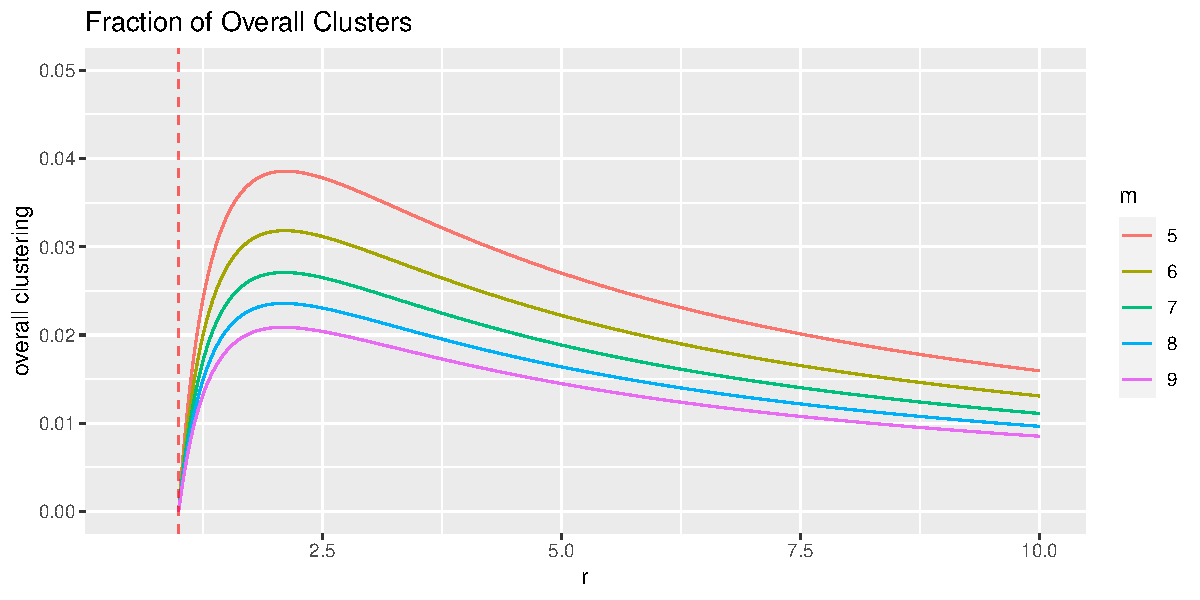
\includegraphics[width=\textwidth]{figures-R/overall-clustering-estimation.pdf}
	\end{center}
	\begin{itemize}
		\item
			In the case where $r\leq1$,
			nodes with very high degree starts to appear and dominates the calculation.
		\item
			So if we want overall clustering,
			we must have $r>1$,
			but not too large.
			\hfill\hyperlink{fig:clustering-estimation}{\beamerreturnbutton{compare to transitive triples}}
	\end{itemize}
\end{frame}

\begin{frame}{Discussion of Clustering}
	\begin{itemize}
		\item
			The choice of which measure of clustering to use is crucial.
		\item
			The meeting-based model can explain clustering,
			there are also other reasons that clustering might emerge:
	\end{itemize}
	\begin{enumerate}
		\item
			Common characteristics among nodes can lead to clustering, e.g.,
			a low connection cost due to geographical reasons.
		\item
			Specifying ``active'' and ``inactive'' nodes can lead to clustering (Klemm \& Egu\'iluz, 2002):
			\begin{itemize}
				\item
					When a new node is born, it is ``active,''
					while one other node turns ``inactive.'' (with probability proportional to inverse degree)
				\item
					A new born node first links to all active nodes,
					then with probability $\mu$,
					each link is rewired to a random node according to preferential attachment.
			\end{itemize}
	\end{enumerate}
\end{frame}

\section{Summary}

\begin{frame}{Summary}
	\begin{itemize}
		\item
			We consider growing networks for two main reasons:
			\begin{enumerate}
				\item It is very natural.
				\item It motivates many properties of real networks.
			\end{enumerate}
		\item
			\textbf{Exponential model} is the natural extension of the Poisson model.
		\item
			\textbf{Preferential attachment model} motives the scale-free distribution.
		\item
			We can model a mix of ``uniformness'' and ``fat-tailedness'' with a \textbf{hybrid model}.
		\item
			Other characteristics such as diameter, assortativity, and clustering can also be motivated by growing networks.
		\item
			The main technical challenge is that even the simplest properties of these networks become increasingly difficult to calculate.
			\textbf{Mean-field approximation} and \textbf{continuous time approximation} are our friends.
	\end{itemize}
\end{frame}

\appendix

\begin{frame}{First-Order Stochastic Dominance}\label{app:FSD}
	\begin{center}
		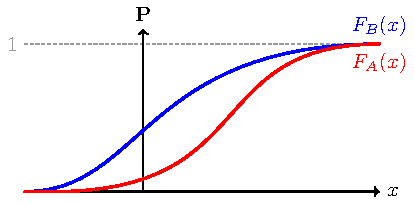
\includegraphics[scale=1]{figures-tikz/stochastic_dominance.pdf}
	\end{center}
	\begin{itemize}
		\item
			Let $A,B$ be two random variables with CDF $F_A$ and $F_B$ respectively.
		\item
			$A$ is said to \textbf{first-order stochastically dominate} $B$ if
			$F_{A}(x)\leq F_{B}(x)$ $\forall x$.
		\item
			It ``dominates'' in the sense that.
			\begin{align*}
				F_{A}(x) \leq F_{B}(x)
				\iff
				\pr{A>x} \geq \pr{B>x}
			\end{align*}
	\end{itemize}
	\hfill\hyperlink{sec:assortativity}{\beamerreturnbutton{back}}
\end{frame}

\end{document}
